
\section{Particle Physics}
Gamma Matrix Identities:
\\
\begin{minipage}{0.45\textwidth}
	\begin{align*}
		\gamma^{0\dagger}&=\gamma^0
		\\
		\gamma^{j\dagger}&=-\gamma^j\quad\qty(j=1,2,3)
		\\
		\gamma^0\gamma^{\mu\dagger}\gamma^0&=\gamma^\mu
		\\
		\gamma^{0}\gamma^{0}&=\mathbb{I}
		\\
		\gamma^\mu\gamma_\mu&=4
		\\
		\gamma^\mu\gamma_\nu\gamma_\mu&=-2\gamma_\nu
		\\
		\gamma^\mu a_\mu&=\gamma_\mu a^\mu=\slsh{a}
		\\
		\psi^\dagger\gamma^0&=\bar{\psi}
	\end{align*}
\end{minipage}
\begin{minipage}{0.48\textwidth}
	\begin{align*}
		\qty{\gamma_\mu,\gamma_\nu}&=\gamma_\mu\gamma_\nu+\gamma_\nu\gamma_\mu=2g_{\mu\nu}
		\\
		\gamma^\mu\gamma_\mu&=4
		\\
		\qty[\gamma^\mu,a_\mu]&=0
		\\
		\gamma^\mu a_\mu&=\gamma_\mu a^\mu=\slsh{a}
		\\
		\Tr(\mathbb{I})&=4
		\\
		\Tr(\gamma_\mu\gamma_\nu)&=\Tr(\gamma^\mu\gamma^\nu)=4
		\\
		\Tr(\gamma_\mu\gamma_\nu\gamma_\rho\gamma_\sigma)&=4(g_{\mu\nu}g_{\rho\sigma}-g_{\mu\rho}g_{\nu\sigma}+g_{\mu\sigma}g_{\nu\rho})
	\end{align*}
\end{minipage}
\\[0.25 cm]
Gamma 5 matrix:
\\
\begin{minipage}{0.45\textwidth}
	\begin{align*}
		\gamma_5^\dagger&=\gamma_5
		\\
		\gamma_{5}\gamma_{5}&=\mathbb{I}
		\\
		\qty{\gamma_5,\gamma_\nu}&=0
		\\
		\Tr(\gamma_5)&=0
		\\
		\Tr(\gamma_\mu\gamma_5)&=0
		\\
		\Tr(\gamma_\mu\gamma_\nu\gamma_5)&=0
		\\
		\Tr(\gamma_\mu\gamma_\nu\gamma_\rho\gamma_5)&=0
		\\
		\Tr(\gamma_\mu\gamma_\nu\gamma_\rho\gamma_\sigma\gamma_5)&=4i\epsilon_{\mu\nu\rho\sigma}
	\end{align*}
\end{minipage}
\begin{minipage}{0.45\textwidth}
	\begin{align*}
		P_L&=\frac{1-\gamma_5}{2}
		\\
		P_R&=\frac{1+\gamma_5}{2}
		\\
		P_L\gamma_\mu&=\gamma_\mu P_R
		\\
		P_L(\gamma^\mu\gamma^\nu\dotsc\text{odd})P_L&=0
		\\
		P_L(\gamma^\mu\gamma^\nu\dotsc\text{even})P_L&=P_L\qty(\gamma^\mu\gamma^\nu\dotsc)
	\end{align*}
\end{minipage}
\\[0.25 cm]
Quick Complex Conjugates:
\\
\begin{align*}
	\qty(\bar{u}\gamma^\mu v)^*&=\bar{v}\gamma^\mu u 
	\\
	\qty(\bar{u}\gamma^\mu P_Lv)^*&=\bar{v}\gamma^\mu P_L u
\end{align*}
\newpage
\begin{comment}
	
	\begin{figure}
		\begin{tikzpicture}
			\feynmandiagram[horizontal=b to d]{
				{a[label=$p_a$],b[label=$p_b$]} -- [fermion] v1 [blob, label=$\vdots$]--[fermion] {c[label=$k_1$],d[label=$k_n$]},
				a -- [opacity=0] b,
				c -- [opacity=0] d,
				};
			\end{tikzpicture}
		\end{figure}
		Mandelstam Variables:
		\tikzfeynmanset{every momentum/arrow shorten/.append style={0.7}}
		\begin{align*}
			\feynmandiagram[baseline=(v1.base), horizontal=v1 to v2]{
				a -- [fermion, momentum'=$p_a$] v1 -- [fermion, reversed momentum=$p_b$] b,
				v1 -- [photon, edge label=$p_a+p_b$] v2 -- [fermion, momentum'=$k_1$] c,
				d -- [fermion, momentum=$k_2$] v2,
				};&& 
				s&=(p_a+p_b)^2c^2=(k_1+k_2)^2c^2
				\\[0.25cm]
				\feynmandiagram[baseline=(v1.base), vertical=v1 to v2]{
					a -- [fermion, momentum'=$p_b$] v1 -- [fermion, momentum=$k_1$] b,
					v1 -- [photon, edge label=$p_a-k_1$] v2 -- [fermion, momentum'=$k_1$] c,
					d -- [fermion, momentum=$p_b$] v2,
					};&& 
					t&=(p_a+p_b)^2c^2=(k_1+k_2)^2c^2
				\end{align*}
			\end{comment}